\begin{bibunit}[IEEEtran.bst]

\chapter*{Introduction}
\addcontentsline{toc}{chapter}{Introduction}
\chaptermark{Introduction}



Understanding and anticipating the ramifications of climate change represents a pressing challenge of our era. Enhancing our knowledge of Earth's systems is a key factor in confronting this challenge.
  Given that the primary source of factual information about the Earth system is observational data, improving our ability to exploit this data could lead to better monitoring and understanding of our planet.
  This thesis focus on the development of methods to exploit satellite observations for improving our knowledge of ocean surface dynamics. 
  More specifically we're asking how advances in deep learning research can be beneficial to ocean observation analysis.
  
  In order to introduce the potentials deep learning for tackling observation problems, we'll introduce the necessary methodological components involved when addressing an observation problem by walking through the development of a thermometer calibration procedure. This simplified problem will help illustrate and contextualize the complementary roles of data and domain knowledge when addressing this class of problem and naturally invite deep learning components in certain aspects of the resolution. 
  
  This will first consist in decomposing the process of mapping the level of the thermometer to the temperature. Then we'll look at the challenges met when evaluating a calibrated thermometer. We'll consider the different sources of errors before finally formalizing the necessary components for developing a thermometer calibration procedure.

  We'll then present how tools brought by deep learning research can contribute to this resolution process and the challenges specific to observation tasks that we can anticipate.

  Finally we'll describe our contributions with the specific observation use-case and the learning-related challenge addressed. 
  
  \section{Calibrating a thermometer}
\subsection{Mapping observations to quantity of interest}
\begin{figure}[h]
    \centering
        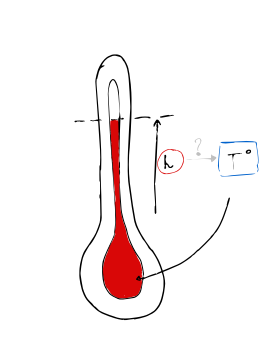
\includegraphics[clip, width=3cm]{Introduction/pics/therm_pb.png}     \\
    \caption{Thermometer Calibration}
    \label{fig:therm_calib}
\end{figure}


When interested in knowing the temperature, we observe the level of a thermometer.
In order to do so, someone had to graduate the thermometer by defining how to map the liquid levels to temperature which can be decomposed in two steps. 

The first step involves accumulating theories and assumptions to construct a model linking the observed level and the actual temperature.
For instance, based on our knowledge of fluid dilation in response to temperature, assuming the diameter of the tube is constant with height, we can posit that the level is linearly correlated with the temperature.
This model introduces two parameters: the slope and offset of our linear model that need to be ascertained.

The second step involves determining these parameters. This step will require some calibration data as inputs. They are traditionally obtained by immersing the thermometer in icing and boiling water to acquire the levels corresponding to 0°C and 100°C.
  Using those data points, a linear system can then be used to solve for the parameters. Which finally gives use our level-to-temperature mapping


The solution, therefore, is a product of both theory and data, and can be reduced to two key components: the model and the algorithm. It demonstrates the importance of balancing abstract concepts with grounded data, and highlights how these two components interplay to produce tools for understanding and interacting with our world.

Interestingly, the model's complexity can often be inversely proportional to the amount of data required. For instance, a model with fewer assumptions demands more data. If we were to abandon the assumption of the thermometer tube's constant diameter, we would need to incorporate a parameterization of the tube diameter in our model. This addition creates more parameters and consequently demands additional data for calibration.

Conversely, having access to more data can allow us to work with fewer assumptions. Suppose we possess a well-calibrated thermometer that can provide unlimited data points. In that case, we could reduce our assumptions to a minimum and rely heavily on empirical evidence, marking each thermometer graduation using data directly from our well-calibrated thermometer.

Lastly, stronger assumptions demand less data. If we introduce the knowledge that the thermometer is immersed in boiling water, our mapping simplifies to a constant function, returning 100°C by convention. This scenario underscores how the incorporation of strong assumptions can drastically reduce the necessity for data.

With these carefully calibrated graduations now etched onto our thermometer, we can use the liquid level as a convenient stand-in for the temperature. However, an important question remains: How can we verify the accuracy of our newly calibrated thermometer?
% A few notes on this example:
% \begin{itemize}
% \item The first step takes in theoretical knowledge and uses a model to output candidate solutions
% \item The second step takes in data and uses an algorithm to output the solution
% \item The solution rely on theory and data and can be reduced to two components model and algorithm.
% \item Fewer assumptions in the model requires more data: If we loosen the assumption about the tube's constant diameter, we need to incorporate a parameterization of the tube diameter into the model, adding more parameters and necessitating additional data for calibration;
% \item More data requires fewer assumptions:If we have a well calibrated thermometer that provides us as many data as we want, we could make very little assumptions and just mark each graduation using data from the calibrated thermometer.
% \item Stronger assumptions requires less data: By adding the knowledge that the thermometer is in boiling water, our mapping is reduced to a constant function returning 100°C by convention.
%   \end{itemize}

% We now have graduations on our thermometer and can use the level as a proxy for the temperature without further thought!... Although how do we know if our calibrated thermometer is any good ? 
\begin{figure}[h]
\centering
\begin{tabular}{ccc}

    Step 1: 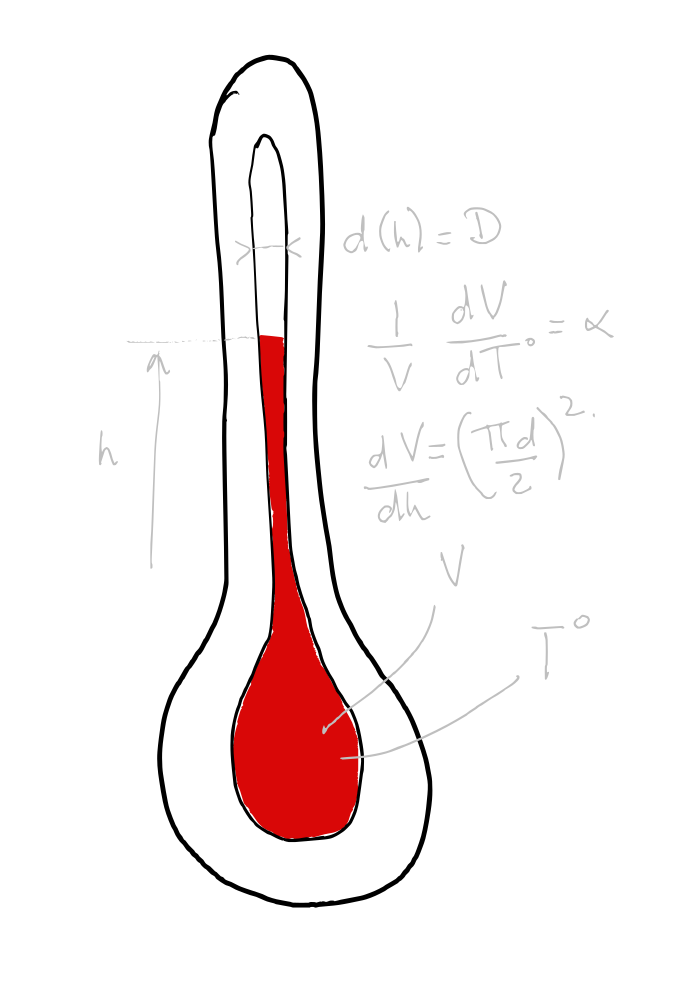
\includegraphics[clip, width=3cm, width=3cm]{Introduction/pics/therm_theroy.png} &    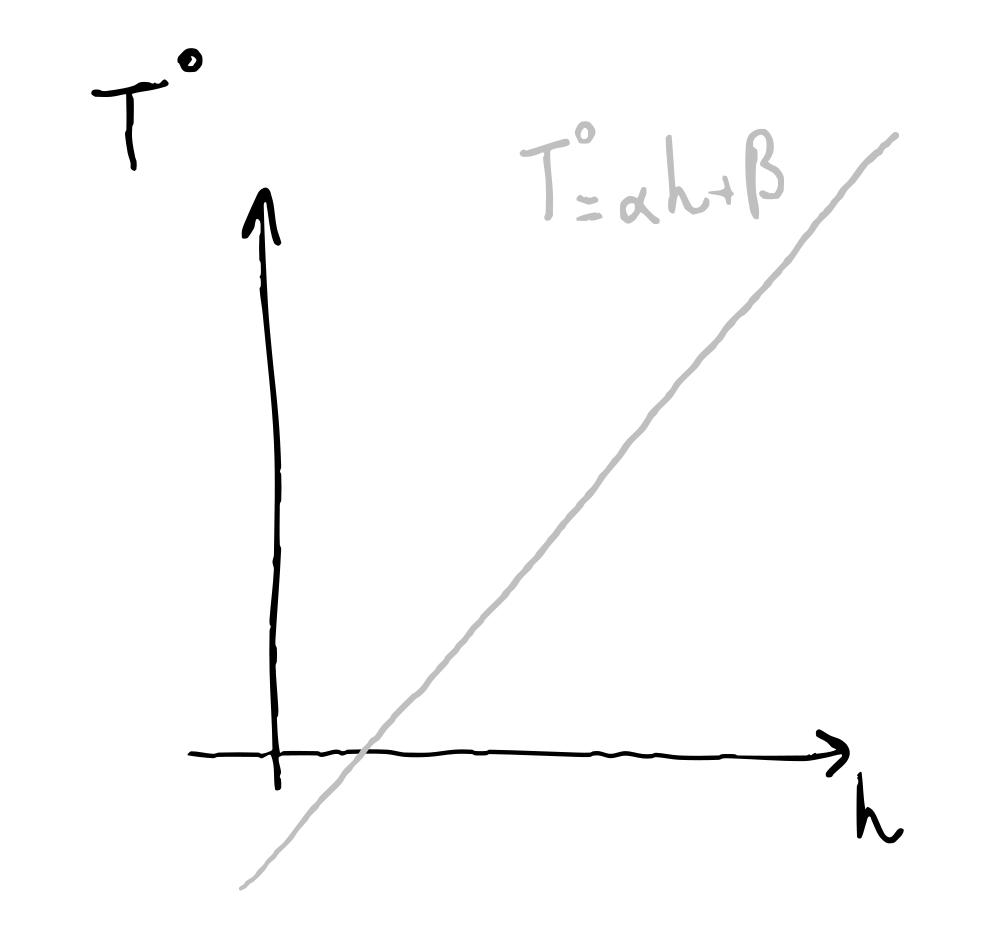
\includegraphics[clip, width=5cm]{Introduction/pics/therm_model.png}     \\  
     Step 2: 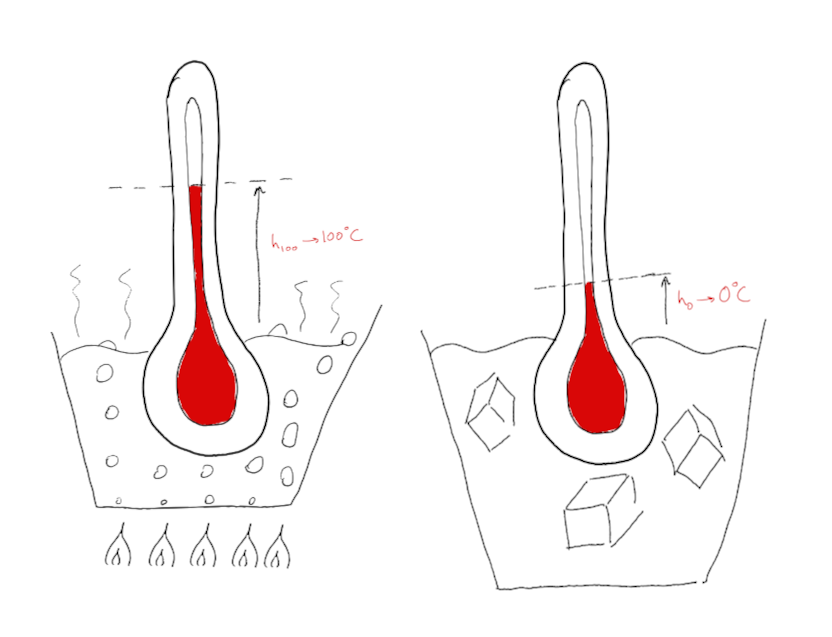
\includegraphics[clip, width=4cm, height=4cm, trim={2cm 1cm 2cm 2cm}]{Introduction/pics/therm_obs.png} &    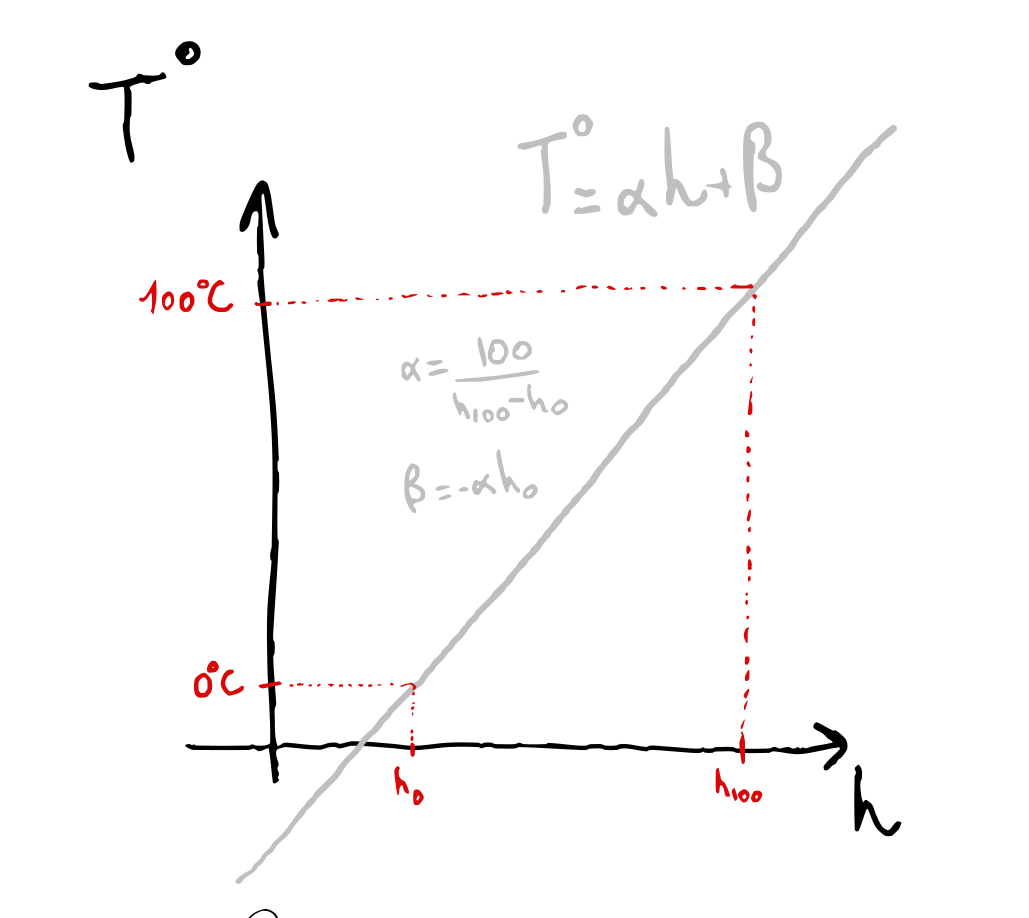
\includegraphics[clip, width=5cm]{Introduction/pics/therm_calib.png}     \\  
\end{tabular}

    \caption{Mapping thermometer level to temperature}
    \label{fig:therm_mapping}
\end{figure}

\subsection{Evaluation}

We define "evaluation" as quantifying quality through metrics.

In our case the most intuitive metric for characterizing our thermometer's quality would be the precision of the temperature it gives.
Note that some situations may put importance on other characteristic such at the range at which it's functional.
  In order to properly evaluate our calibrated instrument, we need to test it in conditions corresponding to its intended use. (testing it domestic thermometer 5000 meter underwater is not not helpful).

 To do so, let's explicit some silent assumptions made on what we expect from our thermometer.
  For example that it needs to "be accurate to the half of degree", "have response time under 10 minutes", "work between -30°C and 200°C" "work at a reasonable atmospheric pressure" etc...

Then we need data to measure the precision of our thermometer in a way that is representative of how we want our thermometer to behave. Using a trustworthy reference like a third-party well-calibrated thermometer, we could compare the measurements of the reference with the one given by our solution.
  An example evaluation procedure could be to confront the measurements of the two instruments at different temperatures such as: in a freezer, in a fridge, at ambiant room temperature and in an oven.

Using the procedure above, we can now compute our metrics and assess if the quality of our calibrated thermometer.
This exercise, however, raises some critical points about evaluation. The process relies on two components that require a deep understanding of the thermometer's intended use: a suitable choice of metric and representative data. If the chosen metrics don't align with the intended use of the thermometer, the evaluation will be flawed. Similarly, if the data isn't representative of the thermometer's intended use, the evaluation will also be flawed.
 Furthermore, the reliability of the reference thermometer is pivotal. If the reference thermometer is not well-calibrated, the best of metrics won't be able to correctly evaluate our thermometer. 

It's also crucial to differentiate between calibration data, which is used to generate a solution, and evaluation data, which is used to assess the solution's quality.
A well-functioning thermometer should provide accurate temperature readings even for levels it wasn't calibrated on. Also, evaluation data should differ from calibration data. If we only measure precision at 0°C and 100°C, a thermometer that perfectly fits the calibration data would receive the highest metric, even if the other graduations are nonsensical.


% Some remarks about the evaluation:
% \begin{itemize}
% \item Evaluation rely on two components, a choice of metric and data
% \item If the metrics' choice are not suited to the intended use of the instrument, the evaluation will be flawed.
% \item If the evaluation data are not representative of the intended use of the instrument, the evaluation will be flawed.
% \item Defining relevant metrics requires intimate knowledge of the intended goal of the instrument.
% \item If the reference thermometer is biased (not well calibrated) a good metric will not define a thermometer of quality
% \item Evaluation and calibration data have different purposes: calibration data is used to give a solution, evaluation data is used to assess the quality of a solution
% \item A good thermometer should give correct temperatures even for levels it were not calibrated on.
% \item Evaluation data should be different than calibration data: If the evaluation only measured the precision at 0°C and 100°C, fitting the calibration data would get the highest metric even if all other graduations were non-sense.
% \item Different metric can produce different rankings, therefore the evaluation is relative to the metric choice
% \item An evaluation can use multiple metrics, therefore no ranking between two methods is guaranteed
% \item Both the single accuracy in the oven and the mean or standard deviations of the different measured accuracies can be considered as metrics
% \end{itemize}


 \subsection{Sources of errors}

Given an evaluation procedure, the errors are the gap to the reference and can be attributed to three sources.

\begin{figure}
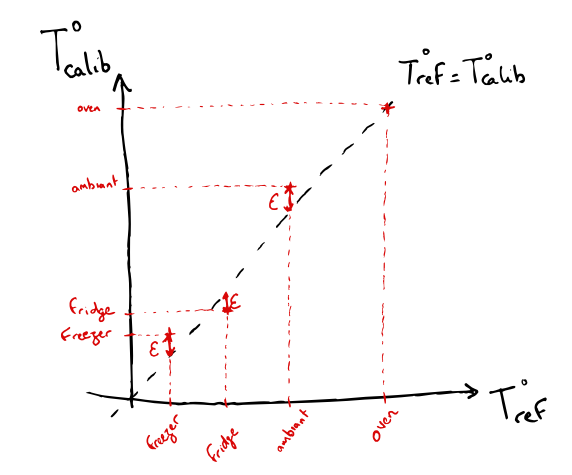
\includegraphics[clip, width=6cm]{Introduction/pics/errors.png}  
\begin{tabular}{c |c|c}

     \hspace{-.15\linewidth}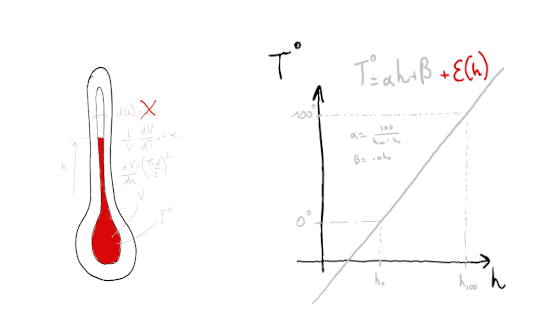
\includegraphics[width=.4\linewidth]{Introduction/pics/model_err_w_source.png}  &
     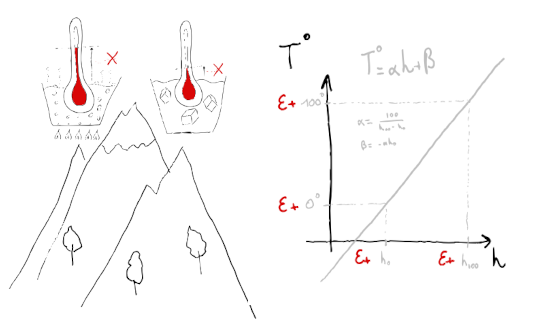
\includegraphics[width=.4\linewidth]{Introduction/pics/data_err_w_source.png} &
     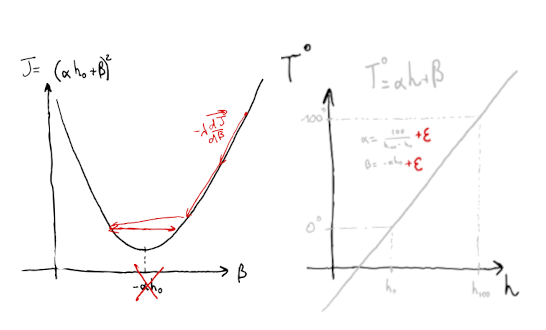
\includegraphics[width=.4\linewidth]{Introduction/pics/optim_err_w_source.png} \\
     \hspace{-.15\linewidth}Model &  Data &  Algorithm \\
\end{tabular}
    \centering
    \caption{Sources of errors}
    \label{fig:err_sources}
\end{figure}
 The model is a source of error if the assumptions made were inaccurate. For example if the diameter of the tube is not constant with height the linear correlation between level and temperature is not exact and will induce errors when interpreting the level.

 Even with perfect assumptions, noisy data can introduce errors in the calibration. If we interpreted our 0°C and 100°C in icing and boiling water at the top of a mountain with lower atmospheric pressure, we will have calibrated our parameters with erroneous measurements and the subsequent graduation of our thermometer will be inaccurate.

 Finally even with perfect assumption and perfect data, the algorithm used to find the solution's parameters can be a source of errors if it fails to find the optimal parameters. For example if we solve for the parameters with a gradient descent method, using a step size too big will prevent finding the exact parameters which will also generate errors in the subsequent measurements.

In order to develop a calibration procedure, we need to take those sources of error into account. The calibration procedure choice will not only depend on the level-temperature relationship but on the whole relationship between calibration data to the final calibrated thermometer. We therefore need to incorporate in our reasoning the how the calibration data was acquired, what is the best model to map the level to the temperature, and what is the best algorithm to find the optimal parameters of the model.

This leads us to the following problem "How to find the best thermometer calibration procedure?"

\subsection{Finding the best thermometer calibration procedure}

We saw previously that to find a solution to the level-temperature mapping problems we have to define a model and an algorithm and have access to calibration data.
Additionally, to evaluate our solution we have to define a metric and have access to evaluation data.

And we detail here how these components can also be specified at a higher level for solving and evaluating the the calibration procedure.


The \textbf{Model} compiles different assumptions to determine the set of candidate calibration procedures.

The \textbf{Algorithm} that is used to chose the best calibration procedure. It can be as trivial as trying out different combination and choosing the best one, or using numerical optimization procedures to determine some higher level parameters. 

The  \textbf{Calibration Data} now needs to be made of calibration tasks with a way to assess the performance of the candidate procedures in order our algorithm to chose the solution.

The \textbf{Evaluation metric} should reflect the intended use of the calibration procedure which includes the range on thermometer on which we would like to use this procedure. An example metric is to use the precision of all the thermometers that we aim to calibrate with the solution.

The \textbf{Evaluation Data} now needs to be representative of the different of the intended use.
Therefore if needs to contain calibration tasks for the variety of thermometers of interest
Furthermore, we need a reference on those tasks to measure the precision on our solution. 



Using those five components, we can select the best calibration procedure, quantify its quality using the evaluation data and use it to calibrate new thermometers and be confident of the resulting calibrated instrument.
We find the parallel between the problems "Finding the level-temperature mapping" and  "Finding the calibration procedure" to be relevant for better understanding further development of this research. We respectively call first order and second order what refers to the former and latter. 




Some remarks about the second order problem
\begin{itemize}
\item A second order solution is a function that takes as inputs first order calibration data and outputs first order solution
\item the evaluation data should still differ from training data for the same reason 
\item Second order parameters can be discrete choices like different first order assumptions "considering the diameter is constant or not"
\item Second order parameters can be discrete choices between two different optimization procedure
\item Second order parameters can be constants in the level-temperature mappings
\item Second order parameters can be parameters of an optimization procedure like step size
\end{itemize}

\section{From thermometer calibration to generic observation problems}
\subsection{Introducing time}
The above calibration infer the temperature of the liquid within the thermometer from its level. One generally uses the thermometer to estimate the temperature of the location where the thermometer is placed.
The response time of the thermometer is the duration before the temperature indicated by the level reflects the temperature of the location it's in. 
If we aimed at knowing the instantaneous temperature of the location of the thermometer, one would need to take into account the temperature change of the liquid. In order to do so multiple observations of the level would be needed.

This observation problem introduce the more generic case of inferring the quantity of interest from a set of observations contrary to the single "thermometer level" used above.

This new problem have repercussions different components of the method/
The evaluation should be carefully designed to measure the dynamical characteristics of the calibration w.r.t the intended use of the thermometer.
The model of this calibration would include additional assumptions and a parameterization of the diffusion process to link the observations to the temperature. This would impact the second order model.
The training data should as well be realigned with the evaluation which would impact the algorithm used to chose the best solution to the problem.

Note that this could be treated as an end to calibration problem if we consider the levels as the thermometer as observations, or as a subsequent problem to the above calibration if we consider the thermometer already graduated and recent observed temperatures as observations. This would impact the different hypothesis made on the model and the noise in the data.


\subsection{Introducing space}
  The objective of the two problems described above is to know the temperature at a single place and time given by the location of the thermometer. 
  This is a particular case of the classes of problem we're interested in.
  The more generic class of problems would be knowing the temperature field over a spatio-temporal domain.

We could then update the associated hierarchy of problems as:
\begin{itemize}
    \item First order problem: Find the field of temperature in a room during a period, given observations of thermometers (potentially at different places and times)
    \item Second order: Determine a procedure that can map a set of observations to the temperature field
\end{itemize}

And the conceptual blocks introduce above apply in a similar manner.

\subsection{The case of satellite altimetry}
  The thermometer provided a good stepping stone to introduce the necessary concepts.
  However the actual problem we're interested in is to estimate the sea surface height (SSH) on the surface of the ocean given satellite data.

  Satellite altimetry which gives us information on the sea surface height (SSH) offers a compelling case study.
  The SSH is related to surface dynamics and current operational products do not resolve processes below 150 km, which are essential for climate monitoring.
  This situation underscores a significant gap in our observational capabilities.
  The recent deployment of a novel sensor during the SWOT satellite mission provides numerous opportunities to address this gap.
  This new sensor introduces unprecedented calibration challenges due to previously unseen errors, but it also promises to enhance the reconstruction of SSH maps.
  As such the contributions of this manuscript explore the application of deep learning to these two observations problems: estimating the SSH from the noisy SWOT observations and estimating the complete SSH field from partial measurements.
  This allows us to formulate the two problems that will be addressed in the manuscript.
  \begin{itemize}
      \item Given scarce calibrated altimetry observations and uncalibrated SWOT observations, estimate the SSH on the domain observed by SWOT
      \item Given scarce SSH observations, estimate the SSH on the whole domain considered
  \end{itemize}
  \begin{figure}
      \centering

          \begin{tabular}{c|c}
            \hspace{-0.2\linewidth}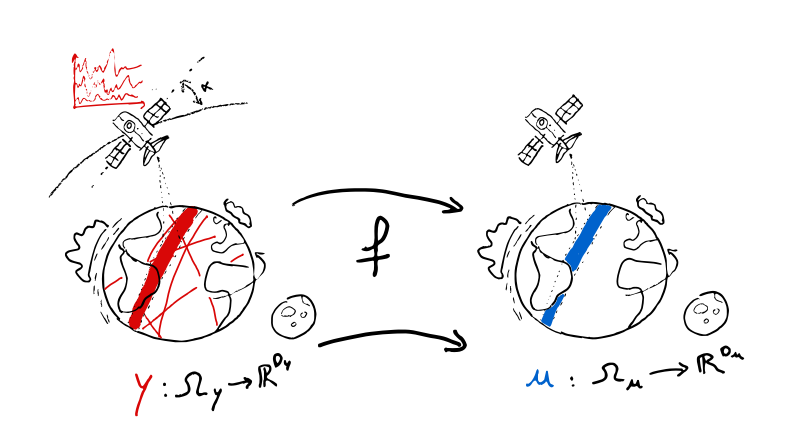
\includegraphics[width=0.7\linewidth]{Introduction/pics/calib_task.png}   & 
            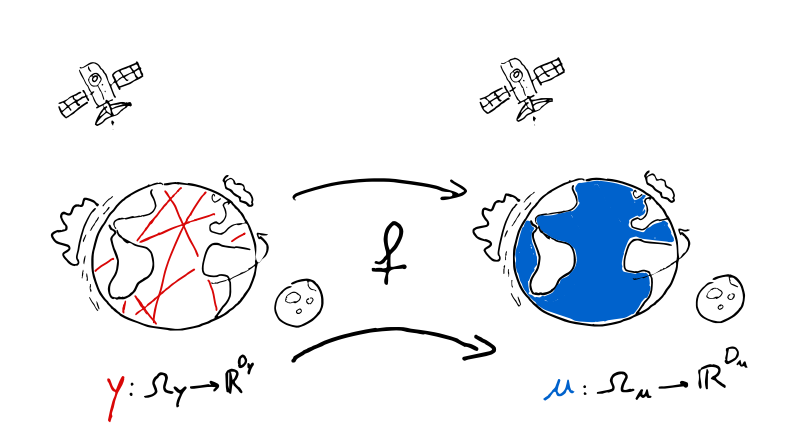
\includegraphics[width=0.7\linewidth]{Introduction/pics/mapping_task.png}\\
           \hspace{-0.2\linewidth} SWOT calibration task & Nadir Altimetry mapping task \\
          \end{tabular}
      \caption{Altimetry observation problems}
      \label{fig:altimetry task}
  \end{figure}

\section{Deep learning potential for altimetry problems}
\subsection{Existing approaches: Model driven versus data driven}

Looking back at remarks of the problem of level-to-thermometer mapping. We noted the feedback loop between model and data.
Under the assumptions that the diameter is constant model of the thermometer, we need two datapoints, If I relax the assumption about the constant diameter and fetch additional data to calibration the new parameters.
On the other hand data driven approaches first frame the problem as an interpolation task and will chose the assumptions that fit the data available.
Given two data points, a reasonable set of candidates to search is the set of linear functions. Given a thousand data points, I can model the mapping with a nearest interpolator effectively reducing my assumptions to stationary (the same level will give the same temperature) and smoothness (the temperature will be close between two levels close by)

Model driven: The strongest assumptions we have the less data we need. The weakest assumptions we have the more data we need.
Data driven: The best data we have, the less assumptions we need. The worst data we have, the more assumptions we need.

\subsection{Deep learning for computer vision and natural language}

Deep learning introduces models with very weak assumptions: neural networks. These models are proven to be able to approximate any function if wide enough. 
A direct consequence is that deep learning models define large sets of possible candidates, requiring consequent datasets and adequate algorithms to find a good solution.
 Many innovation in model architectures such has the ResNet, batchnorms and in optimization procedures with SGD, adam, learning rate schedules kept allowing for searching bigger candidate space and therefore bigger neural networks.
However, the fact that deep learning models can in theory approximate any function introduces a peculiar consideration which is that fitting exactly the calibration data gives you no guarantee on how the model will behave on unseen data. This has standardized the practice of splitting the calibration data in two sets: training and validation. The training set is used  by the optimization procedure to search for the parameters whereas the validation set is used to assess the quality of each candidate. 
The gap of performance between "seen" and "unseen" data is called the generalization gap.
Addressing the problem of generalization have motivated many innovations in regularization, architectures, initialization schemes and data augmentation techniques.


When looking at different application domain, the track records of deep learning in computer vision and natural language are especially impressive. 
The combination of models and algorithm brought by deep learning have managed to solve tasks that previously unsolved.
This can be intuitively understood when considering the challenges of a binary classification task between cats and dogs.
Precisely that the mapping between natural images to binary label is quite difficult to explicitly formalize using domain knowledge. 
The task of predicting the next word of a sentence as done by current LLMs is similarly challenging to model using linguistic theory.

Presented as such deep learning seems to provide universal tools,  
however we would like to stress two factors that seem of great importance when looking at the contributions of deep learning in specific fields.
The first factor is quality and availability of data, indeed the creation of large, curated datasets, like ImageNet in computer vision or ThePile in natural language processing have shown to dramatically expedite the development of novel approaches. 
The second factor is the design of informed architectural patterns that are particularly suited to the domain, leading to performance breakthroughs. Examples of these include convolution techniques and U-Net architectures in computer vision, attention mechanisms in natural language processing.



\subsection{Deep learning for observations}
Compared to other application domain such as CV and NLP, observation problems present a different context for applying deep learning. 
On one hand quite extensive theoretical knowledge have been accumulated on the dynamics that gives structure to the data and that explicitly links the observations with the quantities of interests.  
On the other hand the available data made of observations and numerical model outputs, although consequent, presents challenges since we never have access to the ground truth quantity we want to estimate. (The best we can do is consider a calibrated instrument as ground truth when it's observed). 



This adds
Given a problem stated as above, deep learning brings to the table its set of tools for defining candidate solutions to a problem as well as optimization procedures for searching this set for the optimal candidate.

The main 
Deep learning research keeps demonstrating its potential in exploiting complex structures from data outperforming model driven approaches.
This has been blatant in computer vision over the last decades and in natural language processing over the last years.
Although the progress of deep learning as a generic tool is undeniable when looking at the ever wider range of tasks its applied to.

This manuscript will specifically address these two facets — comprehensive, well-curated datasets and efficient architectural patterns — of deep learning when applied to observation exploitation.

Computer vision and NLP are probably fertile ground for deep learning due to the difficulty of defining models that capture the complex nature of natural language or natural images and that large datasets were accumulated in those fields. 



This constitutes an interesting setup for synergizing physical priors and deep learning models.

Given the 

% \subsection{Model driven, Data driven}
% Looking back at remarks of the problem of level-to-thermometer mapping. We saw the feedback loop between model and data.
% We designate model driven, approaches that first frame the problem as a modelling task and then use the data that fits the assumptions they make of the system.
% Under the assumptions that the diameter is constant model of the thermometer, we need two datapoints, If I relax the assumption about the constant diameter and fetch additional data to calibration the new parameters.
% On the other hand data driven approaches first frame the problem as an interpolation task and will chose the assumptions that fit the data available.
% Given two data points, a reasonable set of candidates to search is the set of linear functions. Given a thousand data points, I can model the mapping with a nearest interpolator effectively reducing my assumptions to stationary (the same level will give the same temperature) and smoothness (the temperature will be close between two levels close by)

% Model driven: The strongest assumptions we have the less data we need. The weakest assumptions we have the more data we need.
% Data driven: The best data we have, the less assumptions we need. The worst data we have, the more assumptions we need.


\subsection{contributions}
More precisely we'll ask wether deep learning can help better exploit satellite observations for improving our knowledge of sea surface dynamics.


Deep learning and earth observation are two well established fields with accumulated knowledge, conventions, and best practices. 
This introduce challenges when developing transdisciplinary approaches that aim to combine expertise from the two fields.
Interfaces need to be proposed to this end which will serve as bridge for domain experts to explore the other side.
Evaluation and data from ocean scientists to ML practicioners. 
Didactic, Generic purpose, and modular implementation of a neural data assimation algorithm for addressing a range of observation problems from ML to ocean



\end{bibunit}

